Add a sound file and play back at a given time, or triggered via OSC
messages.
%
This plugin provides an alternative to the audio player (the
\elem{sndfile} element of \elem{source}).
%
The main difference is, that this plugin loads the whole sound file
into memory, where as the audio player creates a separate jack client
with a decoupling of disk-IO and audio.
%
Offline-rendering is only possible with this audio plugin.

\begin{tscattributes}
  \indattr{name}        & Sound file name.                                                       \\
  \indattr{channel}     & Sound file channel, zero-base (default: 0)                             \\
  \indattr{start}       & Start position within the file, in seconds (default: 0).               \\
  \indattr{length}      & length of sound sample, in seconds, or 0 for file length (default: 0). \\
  \indattr{position}    & Start position within the scene, in seconds (default: 0).              \\
  \indattr{loop}        & loop count or 0 for infinite looping (default: 1).                     \\
  \indattr{levelmode}   & level mode, ``rms'', ``peak'' or ``calib'' (default: ``rms'').         \\
  \indattr{level}       & level in dB (default: 0).                                              \\
  \indattr{triggered}   & Play OSC triggered samples, ignore position and loop (default: false)  \\
  \indattr{transport}   & Use session time base (default: true)                                  \\
  \indattr{license}     & License form of session file                                           \\
  \indattr{attribution} & Attribution of session file, e.g., author name                         \\
  \indattr{mute} & Mute flag\\
\end{tscattributes}

See also Figure \ref{fig:ap_sndfile} for more deatils.

\begin{figure}[htb]
    \centering
    \fbox{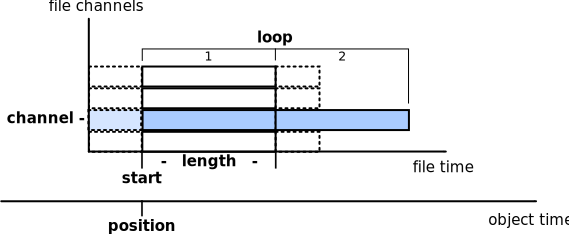
\includegraphics[width=\textwidth]{ap_sndfile}}
    \caption{Explanation of {\tt sndfile} audio plugin attributes.}
    \label{fig:ap_sndfile}
\end{figure}

